\chapter{Implementação e Avaliação}
\label{cp:desenvolvimento}

Este capítulo detalha o processo de implementação prática do \textit{Plot in a Pot}, descrevendo a estrutura física do código, detalhes de componentes e utilitários, testes lógicos de inteligência artificial, benchmarks de desempenho e a metodologia e resultados dos testes de utilizador realizados para validar o sistema.

\section{Estrutura do Código e Detalhes de Implementação}
\label{sec:estrutura-codigo-implementacao}

Para além da fundamentação teórica, o processo de desenvolvimento envolveu a estruturação de uma base de código robusta, modular e altamente reativa. O software está organizado de forma a garantir a separação de conceitos (\textit{Separation of Concerns}), dividindo-se entre componentes de interface visuais, ganchos customizados (\textit{custom hooks}) e utilitários de processamento lógico puro.

\subsection{Gestão de Estado Global, Reatividade e Histórico}
O componente principal \texttt{App.jsx} atua como o orquestrador reativo central do sistema. Para evitar a criação de um ficheiro monolítico, a equipa encapsulou a lógica de negócio em ganchos customizados (\textit{custom hooks}) específicos:
\begin{itemize}
    \item \textbf{\texttt{useSettings}:} Centraliza o estado e a persistência em \textit{LocalStorage} das opções de visualização (ex: exibição de erros, nós secretos, e grau de desfocagem da imagem de fundo).
    \item \textbf{\texttt{useUndoRedo}:} Controla as pilhas de estados anteriores (\texttt{past}) e futuros (\texttt{future}) para as operações atómicas de desfazer e refazer no canvas.
    \item \textbf{\texttt{useChoiceSync}:} Implementa a análise sintática em tempo real para sincronizar as ligações textuais com as arestas correspondentes a escolhas.
    \item \textbf{\texttt{useNodeOperations}:} Encapsula a criação, remoção, duplicação e atualização de propriedades semânticas e posicionais de nós e zonas no editor.
    \item \textbf{\texttt{useGraphHandlers}:} Gere as interações gráficas ligadas ao canvas (ligar nós, atualizar arestas, gerir arrasto e inserção em zonas de agrupamento).
    \item \textbf{\texttt{useKeyboardShortcuts}:} Escuta eventos do teclado para acionar atalhos de produtividade global.
    \item \textbf{\texttt{useProjectPersistence}:} Controla a gravação automática periódica, tradução em tempo real, importação bidirecional de ficheiros Twee 3 e carregamento de modelos base.
\end{itemize}

A implementação do histórico colocou um desafio relevante no contexto de reatividade do React. Como o React Flow atualiza objetos de nós e arestas por referência, a simples inserção de estados na pilha de histórico resultaria na mutação dos estados passados sempre que o utilizador arrastasse um nó. Para resolver esta limitação, implementou-se uma estratégia de clonagem profunda (\textit{deep clone}) em cada instantâneo, conforme demonstrado na Listagem~\ref{lst:app-undo-redo}.

\begin{listing}[H]
\begin{lstlisting}
// Registo de snapshots e funcoes de controlo em useUndoRedo.js
const takeSnapshot = useCallback(() => {
  setPast(prev => [
    ...prev.slice(-50),
    {
      nodes: JSON.parse(JSON.stringify(nodesRef.current)),
      edges: JSON.parse(JSON.stringify(edgesRef.current))
    }
  ]);
  setFuture([]);
}, []);

const undo = useCallback(() => {
  if (past.length === 0) return;
  const previous = past[past.length - 1];
  setFuture(prev => [
    {
      nodes: JSON.parse(JSON.stringify(nodesRef.current)),
      edges: JSON.parse(JSON.stringify(edgesRef.current))
    },
    ...prev
  ]);
  setPast(prev => prev.slice(0, -1));
  setNodes(previous.nodes);
  setEdges(previous.edges);
}, [past]);
\end{lstlisting}
\caption{Mecanismo de clonagem profunda e gestão da pilha de histórico encapsulado em useUndoRedo.js.}
\label{lst:app-undo-redo}
\end{listing}

Esta estrutura suporta o fluxo reativo unidirecional da aplicação. Quando o autor edita o texto de uma passagem no painel de propriedades, um evento de alteração é propagado para o estado central em \texttt{App.jsx}, que força a reavaliação síncrona e em segundo plano de dois subsistemas independentes: o parser de texto (que extrai as novas arestas baseadas em ligações double-bracket e reconstrói a Lista de Adjacência em memória) e o validador estático (que executa a travessia BFS sobre a nova lista de adjacência para detetar inconsistências e desenhar alertas visuais de aviso diretamente no canvas).

\subsection{Componentes Gráficos e Desafios de Interação (Canvas, Nós e Arestas)}
Os nós gráficos que habitam o canvas estendem os componentes base da biblioteca React Flow (conforme ilustrado na Figura~\ref{fig:editor-canvas}):
\begin{itemize}
    \item \textbf{StoryNode.jsx:} Renderiza o título da passagem, o extrato de texto da história e as portas de ligação (\textit{handles}) de entrada e saída.
    \item \textbf{ZoneNode.jsx (Agrupamento Visual):} Implementa o agrupamento de capítulos. Para resolver o conflito de eventos de rato (onde a Zona sobreposta impedia cliques no canvas de fundo ou nos nós filhos), aplicou-se a propriedade CSS \texttt{pointer-events: none} ao contêiner geral da Zona, e ativou-se \texttt{pointer-events: all} exclusivamente para as bordas de redimensionamento e barra de cabeçalho, como demonstrado na Listagem~\ref{lst:zone-pointer-events}.
    \item \textbf{EditableEdge.jsx (Arestas Curvas):} Implementa o traçado curvo interativo. O utilizador pode efetuar um duplo clique sobre a linha para introduzir um ponto de controlo (\textit{waypoint}) geométrico. O algoritmo (Listagem~\ref{lst:edge-path-svg}) interpola os pontos e converte a spline Catmull-Rom em comandos de curva Bézier cúbica SVG (\texttt{C}) compatíveis com o navegador.
\end{itemize}

\begin{figure}[H]
    \centering
    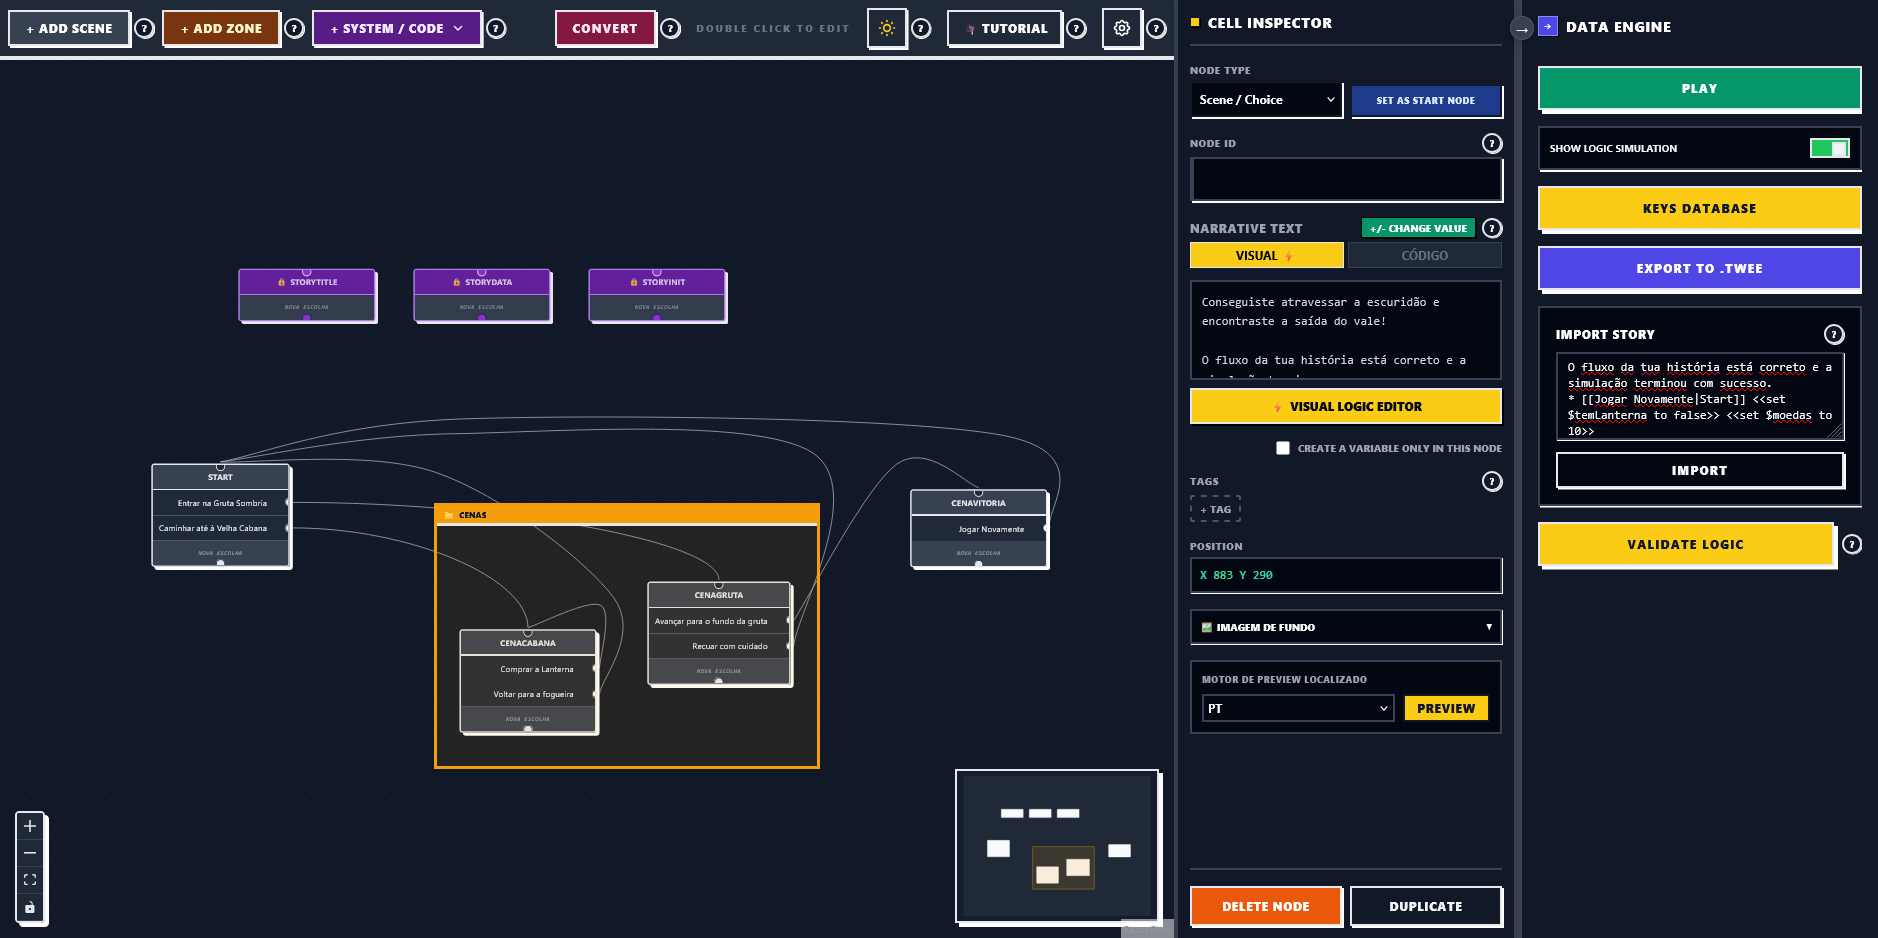
\includegraphics[width=0.85\linewidth]{Figures/editor_canvas.png}
    \caption{Interface gráfica do canvas de grafos do Plot in a Pot, demonstrando a estética neo-brutalista de alto contraste com nós de cena e agrupamentos visuais (Zonas).}
    \label{fig:editor-canvas}
\end{figure}

\begin{listing}[H]
\begin{lstlisting}
<!-- Estrutura simplificada do componente ZoneNode -->
<div 
  className="zone-node-container" 
  style={{ pointerEvents: 'none' }}
>
  <div 
    className="zone-node-header" 
    style={{ pointerEvents: 'all' }}
  >
    <h3>{data.title}</h3>
  </div>
  <div 
    className="zone-node-body" 
    style={{ border: '2px dashed #000' }}
  >
    {/* Os nos filhos sao renderizados no topo e respondem a cliques */}
  </div>
</div>
\end{lstlisting}
\caption{Resolução de eventos de rato através de regras CSS em ZoneNode.jsx.}
\label{lst:zone-pointer-events}
\end{listing}

\begin{listing}[H]
\begin{lstlisting}
// Geracao da curva SVG com interpolacao de pontos geometricos
export function getCatmullRomPath(points) {
  if (points.length < 2) return '';
  let path = `M ${points[0].x} ${points[0].y}`;
  for (let i = 0; i < points.length - 1; i++) {
    const p0 = points[i - 1] || points[i];
    const p1 = points[i];
    const p2 = points[i + 1];
    const p3 = points[i + 2] || p2;
    
    // Calculo dos pontos de controlo Bezier baseados em Catmull-Rom
    const cp1x = p1.x + (p2.x - p0.x) / 6;
    const cp1y = p1.y + (p2.y - p0.y) / 6;
    const cp2x = p2.x - (p3.x - p1.x) / 6;
    const cp2y = p2.y - (p3.y - p1.y) / 6;
    
    path += ` C ${cp1x} ${cp1y}, ${cp2x} ${cp2y}, ${p2.x} ${p2.y}`;
  }
  return path;
}
\end{lstlisting}
\caption{Algoritmo de interpolação e desenho de curvas no componente EditableEdge.jsx.}
\label{lst:edge-path-svg}
\end{listing}

\subsection{Mapeamento Reverso, Expressões Regulares e Matriz de Localização}
Para gerir a complexidade de narrativas extensas, a equipa implementou as seguintes soluções:
\begin{itemize}
    \item \textbf{Mapeamento Reverso no Inspector:} O painel lateral \texttt{Inspector.jsx} lê e sincroniza os dados do nó selecionado. Para evitar que o autor tenha de inspecionar visualmente todo o canvas, o componente realiza um mapeamento reverso sobre a lista de adjacências para identificar e expor em tempo real todos os caminhos incidentes de entrada e saída (Listagem~\ref{lst:inspector-adjacency}).
    \item \textbf{Refatorização de Variáveis em VariablesModal:} Quando o utilizador renomeia uma variável global, o sistema varre e atualiza de forma atómica todas as ocorrências em todos os nós da história. A substituição recorre a uma expressão regular compilada com barreira de palavras (\texttt{\textbackslash b}) para evitar sobreposição de nomes parciais (conforme a Figura~\ref{fig:variables-modal} e Listagem~\ref{lst:variables-regex}).
    \item \textbf{Matriz de Localização e Parser CSV:} O painel \texttt{TranslationMatrix.jsx} expõe uma grelha de tradução (ilustrada na Figura~\ref{fig:translation-matrix}). Para permitir a interoperabilidade com editores de folhas de cálculo externos, desenvolveu-se um parser de importação \gls{csv} personalizado aderente à norma RFC 4180 (Listagem~\ref{lst:translation-csv}).
\end{itemize}

\begin{listing}[H]
\begin{lstlisting}
// Calculo de caminhos incidentes no painel lateral
const getConnections = (nodeId, edges, nodes) => {
  const incoming = edges
    .filter(edge => edge.target === nodeId)
    .map(edge => {
      const srcNode = nodes.find(n => n.id === edge.source);
      return { id: edge.source, label: srcNode?.data?.label || edge.source };
    });
    
  const outgoing = edges
    .filter(edge => edge.source === nodeId)
    .map(edge => {
      const tgtNode = nodes.find(n => n.id === edge.target);
      return { id: edge.target, label: tgtNode?.data?.label || edge.target };
    });
    
  return { incoming, outgoing };
};
\end{lstlisting}
\caption{Mapeamento dinâmico de nós predecessores e sucessores em Inspector.jsx.}
\label{lst:inspector-adjacency}
\end{listing}

\begin{listing}[H]
\begin{lstlisting}
// Substituicao em lote de variaveis nos textos dos nos
const refactorVariableInNodes = (oldName, newName, currentNodes) => {
  const escapedOld = oldName.replace(/[-\/\\^$*+?.()|[\]{}]/g, '\\$&');
  const regex = new RegExp(escapedOld + '\\b', 'g');
  
  return currentNodes.map(node => {
    const text = node.data.content || '';
    if (regex.test(text)) {
      return {
        ...node,
        data: { ...node.data, content: text.replace(regex, newName) }
      };
    }
    return node;
  });
};
\end{lstlisting}
\caption{Refatorização automática de variáveis lógicas baseada em \gls{regex} no VariablesModal.jsx.}
\label{lst:variables-regex}
\end{listing}

\begin{listing}[H]
\begin{lstlisting}
// Conversao de texto CSV bruto numa matriz de traducao
const parseCSVToTranslations = (csvText) => {
  const rows = [];
  let currentRow = [];
  let currentCell = '';
  let inQuotes = false;
  
  for (let i = 0; i < csvText.length; i++) {
    const char = csvText[i];
    const nextChar = csvText[i + 1];
    
    if (char === '"') {
      if (inQuotes && nextChar === '"') {
        currentCell += '"';
        i++;
      } else {
        inQuotes = !inQuotes;
      }
    } else if (char === ',' && !inQuotes) {
      currentRow.push(currentCell.trim());
      currentCell = '';
    } else if ((char === '\n' || char === '\r') && !inQuotes) {
      if (char === '\r' && nextChar === '\n') i++;
      currentRow.push(currentCell.trim());
      rows.push(currentRow);
      currentRow = [];
      currentCell = '';
    } else {
      currentCell += char;
    }
  }
  return rows;
};
\end{lstlisting}
\caption{Parser de importação de ficheiros \gls{csv} com suporte à norma RFC 4180 em TranslationMatrix.jsx.}
\label{lst:translation-csv}
\end{listing}

\begin{figure}[H]
    \centering
    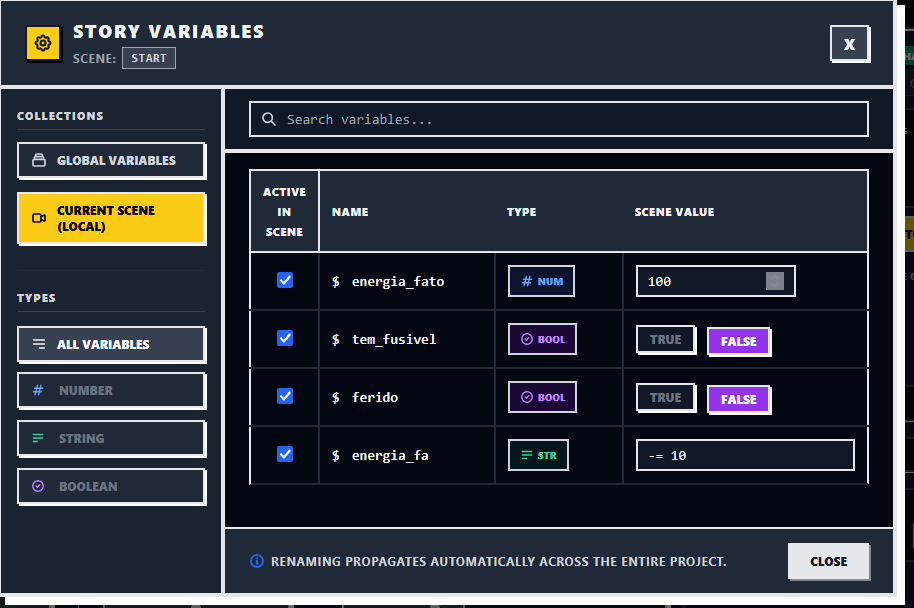
\includegraphics[width=0.85\linewidth]{Figures/variables_modal.png}
    \caption{Diálogo de gestão de variáveis globais (VariablesModal), apresentando os tokens de dados e a renomeação segura baseada em \gls{regex}.}
    \label{fig:variables-modal}
\end{figure}

\begin{figure}[H]
    \centering
    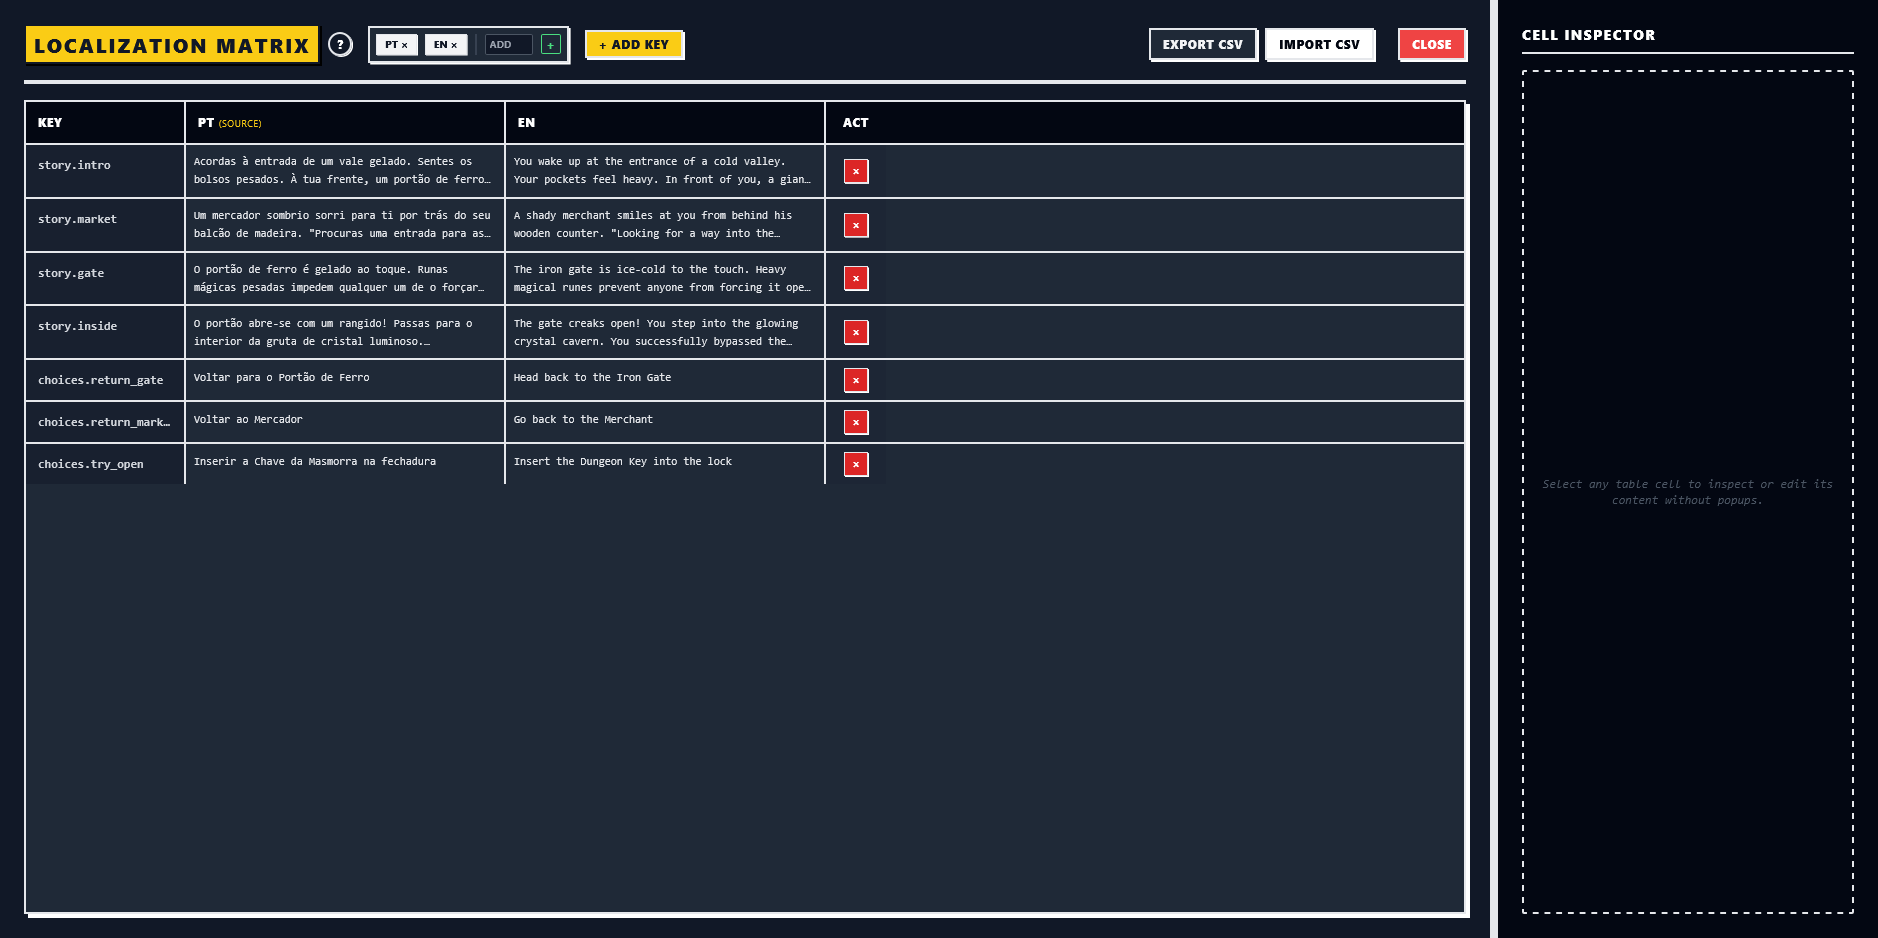
\includegraphics[width=0.85\linewidth]{Figures/translation_matrix.png}
    \caption{Matriz de localização integrada no editor, exibindo a grelha de chaves de texto e a respetiva tradução direta para os idiomas selecionados.}
    \label{fig:translation-matrix}
\end{figure}

\subsection{Sandbox de Simulação, Edição Lógica Estruturada e Utilitários}
Para além dos componentes gráficos, a equipa implementou módulos de simulação, edição estruturada de lógica e processamento sintático puro (que operam fora do ciclo de renderização direta do DOM):
\begin{itemize}
    \item \textbf{PlayMode.jsx (Sandbox Isolada):} Mimetiza a execução da história. Para evitar que variáveis de script globais escritas pelo utilizador interfiram com os estados internos da aplicação React, o motor executa os blocos dinâmicos sob uma sandbox isolada baseada no construtor de funções dinâmicas (como exibido na Figura~\ref{fig:playmode-simulation} e Listagem~\ref{lst:playmode-sandbox}).
    \item \textbf{VisualBlocksEditor.jsx (Edição Estruturada):} Permite que autores configurem prosa, setters de variáveis e escolhas condicionais graficamente, as quais são convertidas em macros SugarCube (apresentada na Figura~\ref{fig:visual-blocks} e Listagem~\ref{lst:visual-blocks}).
    \item \textbf{tweeParser.js (Parser de Layout):} Converte o canvas reativo em ficheiro de texto Twee 3. O parser processa as coordenadas posicionais, convertendo-as de absolutas para relativas caso os nós estejam contidos em Zonas de Agrupamento (Listagem~\ref{lst:parser-coordinate-conversion}).
    \item \textbf{storyTraversal.js e storyValidator.js (Validador BFS):} Executa a travessia de espaço de estados. A Listagem~\ref{lst:traversal-loop} ilustra o ciclo principal do algoritmo, evidenciando a paragem reguladora de segurança de visitas a nós a um limite $K = 10$ estados lógicos distintos.
    \item \textbf{aiGenerator.js (Assistente de Conversão com IA):} Efetua chamadas assíncronas HTTP REST para o servidor Ollama na porta padrão, estruturando prompts de sistema para desativar saídas coloquiais e garantir o formato Twee 3 (Listagem~\ref{lst:ai-request}).
\end{itemize}

\begin{listing}[H]
\begin{lstlisting}
// Execucao controlada de scripts do utilizador
const executeScriptInSandbox = (scriptContent, gameState) => {
  try {
    const sandbox = new Function('state', `
      with(state) {
        ${scriptContent}
      }
    `);
    const stateClone = JSON.parse(JSON.stringify(gameState));
    sandbox(stateClone);
    return stateClone;
  } catch (error) {
    console.error("Erro na execucao do script:", error);
    return gameState;
  }
};
\end{lstlisting}
\caption{Mecanismo de execução de scripts de lógica com isolamento de contexto no PlayMode.jsx.}
\label{lst:playmode-sandbox}
\end{listing}

\begin{listing}[H]
\begin{lstlisting}
// Conversao de logica estruturada em texto de macros SugarCube
export function serializeLogicToText(logic) {
  const parts = [];
  if (logic.narrative) {
    parts.push(logic.narrative);
    parts.push('');
  }
  if (logic.setters && logic.setters.length > 0) {
    logic.setters.forEach(s => {
      if (s.variable.trim()) {
        parts.push(`<<set $${s.variable.trim()} to ${s.value}>>`);
      }
    });
    parts.push('');
  }
  return parts.join('\n');
}
\end{lstlisting}
\caption{Serialização da estrutura de formulários lógicos em macros SugarCube (logicParser.js).}
\label{lst:visual-blocks}
\end{listing}

\begin{figure}[H]
    \centering
    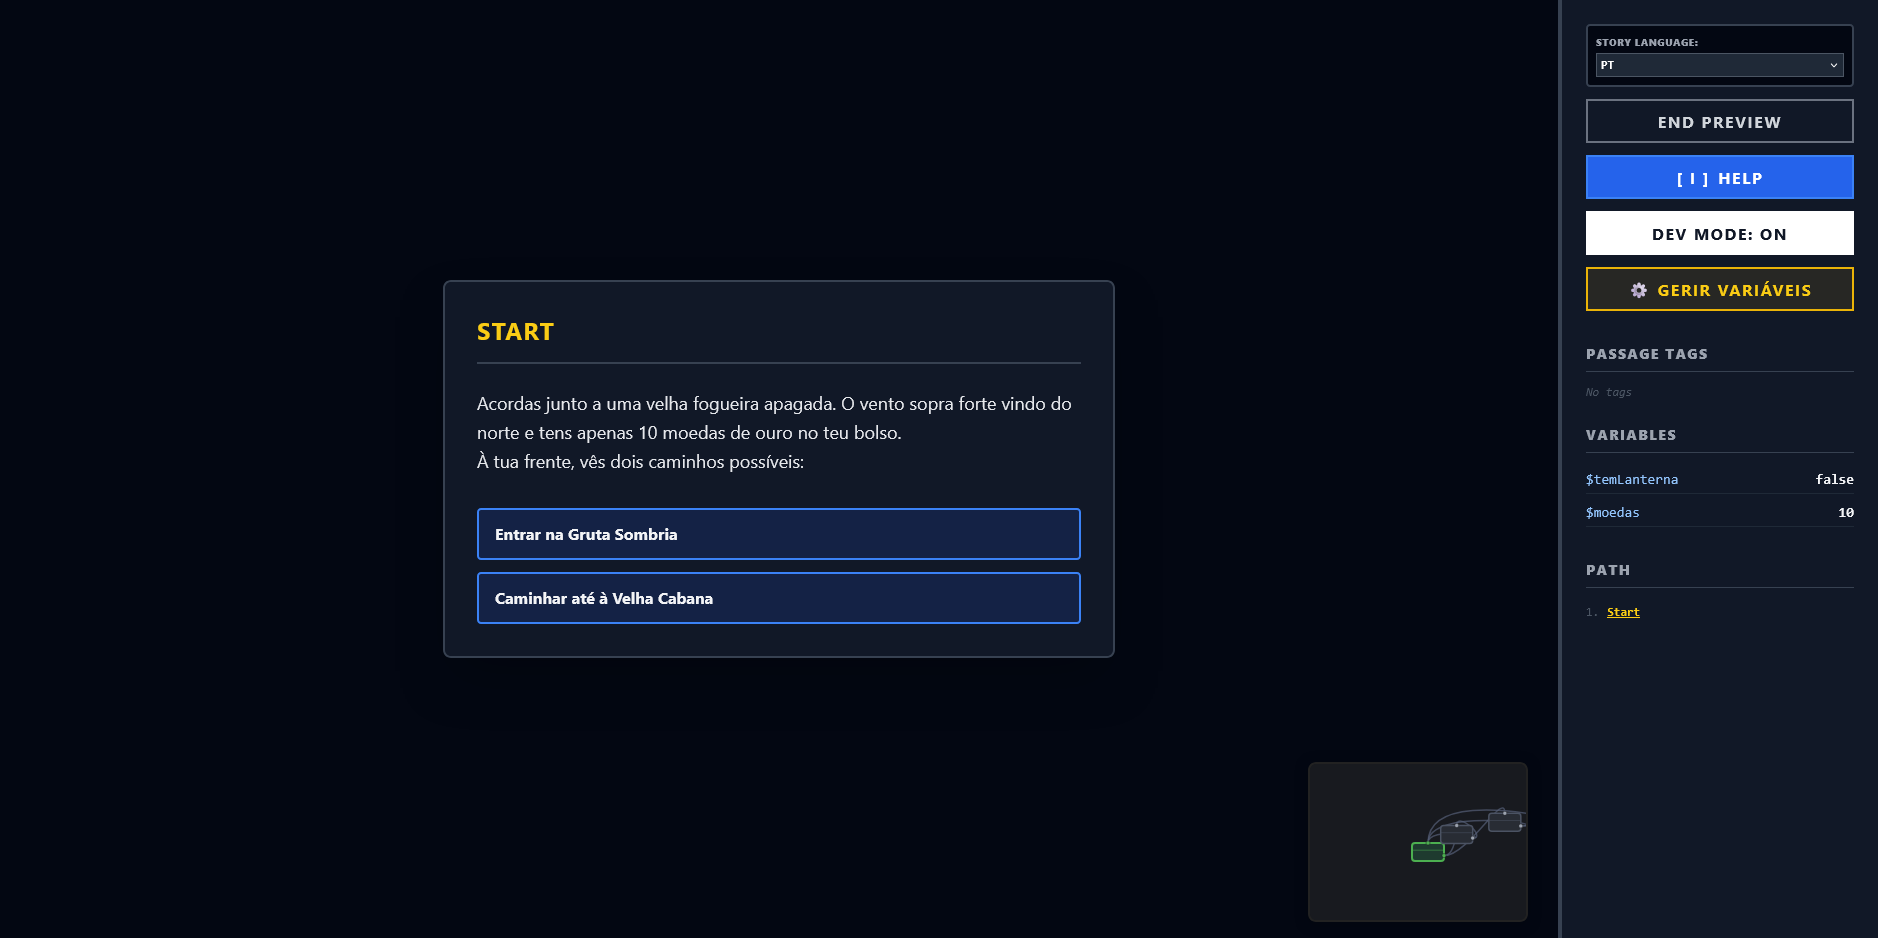
\includegraphics[width=0.85\linewidth]{Figures/playmode_simulation.png}
    \caption{Ecrã da sandbox de simulação (PlayMode), ilustrando a execução em tempo real da história com o painel de depuração de variáveis lógicas.}
    \label{fig:playmode-simulation}
\end{figure}

\begin{figure}[H]
    \centering
    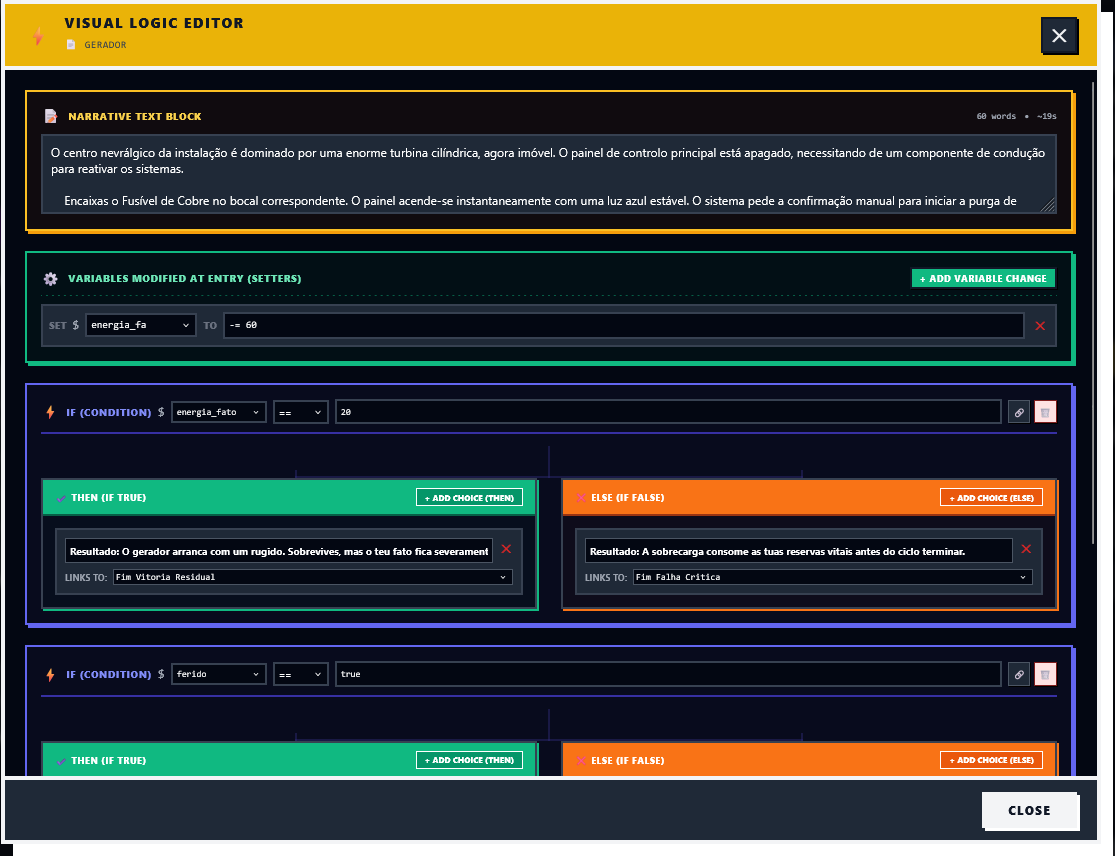
\includegraphics[width=0.85\linewidth]{Figures/visual_blocks.png}
    \caption{Interface do editor visual de lógica estruturada (VisualBlocksEditor), dividindo as passagens em painéis de prosa, setters de variáveis e escolhas condicionais.}
    \label{fig:visual-blocks}
\end{figure}

\begin{listing}[H]
\begin{lstlisting}
// Conversao de coordenadas na leitura de passagens Twee 3
export function parsePassageMetadata(metaString, zoneMap) {
  try {
    const meta = JSON.parse(metaString || '{}');
    let x = meta.position?.x ?? 0;
    let y = meta.position?.y ?? 0;
    const parentId = meta.parentId;
    
    if (parentId && zoneMap.has(parentId)) {
      const zone = zoneMap.get(parentId);
      x = x - (zone.position?.x ?? 0);
      y = y - (zone.position?.y ?? 0);
    }
    return { x, y, parentId, width: meta.size?.width, height: meta.size?.height };
  } catch (e) {
    return { x: 0, y: 0 };
  }
}
\end{lstlisting}
\caption{Processamento de coordenadas absolutas e relativas de nós e Zonas em tweeParser.js.}
\label{lst:parser-coordinate-conversion}
\end{listing}

\begin{listing}[H]
\begin{lstlisting}
// Travessia e controlo de ciclos por limite de estados visitados
while (queue.length > 0) {
  const { nodeId, state, path } = queue.shift();
  const currentNode = nodeMap.get(nodeId);
  if (!currentNode) continue;
  
  const newState = applyModifiers(currentNode.data.content, state);
  const stateStr = JSON.stringify(newState);
  
  if (!visitedStates.has(nodeId)) visitedStates.set(nodeId, []);
  if (visitedStates.get(nodeId).includes(stateStr)) continue;
  
  if (visitedStates.get(nodeId).length >= 10) {
    console.warn(`Ciclo infinito provavel no no ${currentNode.data.label}`);
    continue;
  }
  
  visitedStates.get(nodeId).push(stateStr);
  arrivalHistory.get(nodeId).push({ path, state: newState });
}
\end{lstlisting}
\caption{Ciclo principal de exploração do espaço de estados no motor storyTraversal.js.}
\label{lst:traversal-loop}
\end{listing}

\begin{listing}[H]
\begin{lstlisting}
// Envio do prompt de conversao estrutural para o Ollama local
export async function generateTweeFromText(userText, modelName = 'llama3') {
  const response = await fetch('http://localhost:11434/api/chat', {
    method: 'POST',
    headers: { 'Content-Type': 'application/json' },
    body: JSON.stringify({
      model: modelName,
      messages: [
        { role: 'system', content: 'You are a parser. Convert the story to Twee 3. Output ONLY raw Twee 3 format.' },
        { role: 'user', content: userText }
      ],
      stream: false
    })
  });
  const data = await response.json();
  return data.message?.content || '';
}
\end{lstlisting}
\caption{Estrutura de comunicação assíncrona com o Ollama local em aiGenerator.js.}
\label{lst:ai-request}
\end{listing}

\section{Testes de Conversão e Comparação de Modelos de Linguagem (IA Local)}

Para analisar a viabilidade do assistente de importação de texto livre, foram realizados testes com diferentes modelos de linguagem (\glspl{llm}) executados localmente. A escolha do ecossistema Ollama para estes testes justifica-se por ser uma ferramenta leve e otimizada de orquestração local que expõe uma API REST padrão, facilitando a integração direta com o editor e assegurando a soberania dos dados sem custos de operação.

\subsection{Primeira Fase: Testes em Máquina Local (RTX 3050)}
A primeira série de testes foi realizada a 9 de maio no computador do programador, equipado com uma placa gráfica Nvidia RTX 3050 (Laptop) com 4\,GB de VRAM. O objetivo do teste consistiu em submeter uma narrativa linear escrita em linguagem natural para avaliar a capacidade do modelo em estruturar as passagens e os respetivos caminhos de ligação conformes à sintaxe Twee 3. Selecionaram-se os seguintes modelos locais da biblioteca Ollama:
\begin{itemize}
    \item Gemma 2B: ID \texttt{8ccf136fdd52}
    \item Mistral 7B: ID \texttt{6577803aa9a0}
    \item Qwen 3.5 9B: ID \texttt{6488c96fa5fa}
    \item DeepSeek Coder 6.7B: ID \texttt{ce298d984115}
\end{itemize}
Além destes, foi testado o modelo Claude (acessível via API externa). Contudo, devido às restrições severas de memória da placa gráfica local de 4\,GB, nenhum dos modelos locais funcionou adequadamente, gerando lentidão extrema no sistema operativo e erros de falta de memória (\textit{out of memory}).

\subsection{Segunda Fase: Testes com Maior Capacidade de Processamento}
Para viabilizar a execução e avaliação comparativa dos modelos locais, a 19 de maio realizaram-se os mesmos testes num servidor de desenvolvimento equipado com uma GPU Nvidia Titan Xp com 12\,GB de VRAM. A análise das respostas obtidas revelou falhas sistemáticas em cada modelo que inviabilizaram a importação direta:
\begin{itemize}
    \item \textbf{Mistral 7B (\texttt{mistral\_7b}):} O resultado revelou-se inadequado para a aplicação. O modelo separou quase todas as frases do texto em passagens independentes, gerando dezenas de pequenos nós para uma única cena, o que corrompeu o fluxo e a legibilidade do grafo. Adicionalmente, inseriu barras invertidas no final das linhas e lixo de terminal (como sequências de controlo ANSI). Posteriormente, identificou-se que esta poluição de caracteres se deveu ao modo como a ferramenta de linha de comandos (CLI) do Ollama lida com saídas direcionadas em processos automáticos sem terminal interativo (TTY), problema este contornável através da utilização de uma API REST ou via scripts Python.
    \item \textbf{Gemma 4B / 2B (\texttt{gemma4\_e4b}):} O modelo esboçou a criação de passagens, mas inseriu os cabeçalhos de definição de passagem (o marcador \texttt{::}) no interior do corpo de texto de outros nós. Sendo que a especificação Twee 3 proíbe passagens aninhadas, o parser interpretou a totalidade da resposta como um único nó corrompido.
    \item \textbf{Qwen 3 8B (\texttt{qwen3\_8b}):} O resultado revelou-se inutilizável pois o modelo incluiu os seus blocos de raciocínio interno (prefixados por \textit{``Thinking...''}) no início da resposta, inviabilizando o parsing. Adicionalmente, gerou um bloco JSON incompleto e caracteres ANSI no fluxo de texto.
    \item \textbf{Qwen 3.5 9B (\texttt{qwen3.5\_9b}):} Apresentou o melhor desempenho de mapeamento e estrutura formal de caminhos, mas ainda assim falhou na conformidade total devido à inclusão de textos de raciocínio intermediário no início da resposta e à geração de nós órfãos desconetados da árvore principal.
\end{itemize}

\subsection{Identificação do Bug Técnico no Ollama}
Mais tarde, identificou-se que a presença de lixo do terminal (códigos ANSI, sequências \texttt{[3D [K}, etc.) se deve a um comportamento documentado do CLI do Ollama (Issue \#14571 no GitHub). Quando o utilitário \texttt{ollama run} é invocado programaticamente a partir de um processo em segundo plano, ele falha em detetar a ausência de um terminal interativo (TTY), continuando a injetar caracteres de escape ANSI de controlo de cursor na resposta textual.

Para mitigar este problema no \gls{piap}, identificaram-se três abordagens corretivas:
\begin{enumerate}
    \item \textbf{Limpeza com Expressões Regulares:} Filtrar o texto de saída na aplicação aplicando uma expressão regular para expurgar as sequências ANSI.
    \item \textbf{Descartar a Saída de Erros:} Redirecionar o fluxo de erro padrão (\texttt{stderr}) do processo do Ollama para o nulo.
    \item \textbf{Uso da API REST do Ollama (Implementada):} Ligar a aplicação diretamente à API HTTP REST local do Ollama (na porta \texttt{11434}). A API REST contorna o CLI oficial e devolve o texto limpo de formatação.
\end{enumerate}

\subsection{Estado Atual da Funcionalidade (Beta) e Trabalho Futuro}
Conclui-se que o modelo Qwen 3.5 9B apresenta a melhor estrutura narrativa e conformidade com o parser. No entanto, mesmo com acesso a hardware dedicado com capacidade superior a 8\,GB de VRAM, a funcionalidade de conversão por IA local permanece em fase experimental (beta), uma vez que a precisão de mapeamento estrutural e a correta filtragem de blocos de raciocínio interno (como tags \texttt{<think>...</think>}) exigem novos refinamentos de prompting e de filtros prévios de processamento. Esta funcionalidade constitui uma linha de investigação ativa para futuros desenvolvimentos.

\section{Análise de Desempenho e Complexidade Algorítmica}
\label{sec:analise-desempenho-complexidade}

Para validar a conformidade da aplicação com o requisito não-funcional de fluidez e desempenho (RNF03), que estipula latências de interação inferiores a 100 milissegundos, realizou-se uma avaliação da complexidade teórica e do comportamento prático do software sob diferentes cargas de dados.

\subsection{Complexidade Algorítmica Teórica}
Os módulos de cálculo do \textit{Plot in a Pot} operam de forma síncrona no lado do cliente. A Tabela~\ref{tab:complexidade-teorica} resume a complexidade temporal e espacial assintótica (na notação Big-$\mathcal{O}$) dos três algoritmos mais exigentes em termos computacionais.

\begin{table}[H]
\centering
\caption{Complexidade algorítmica teórica dos subsistemas nucleares.}
\label{tab:complexidade-teorica}
\begin{tabularx}{\textwidth}{LCC}
\toprule
\textbf{Subsistema / Algoritmo} & \textbf{Complexidade Temporal} & \textbf{Complexidade Espacial} \\
\midrule
Parser Bidirecional Twee 3 & $\mathcal{O}(L)$ & $\mathcal{O}(V + E)$ \\
Validador de Espaço de Estados (\gls{bfs}) & $\mathcal{O}(V + E \cdot K)$ & $\mathcal{O}(V \cdot K + E)$ \\
Interpolação de Arestas (Catmull-Rom) & $\mathcal{O}(W)$ & $\mathcal{O}(W)$ \\
\bottomrule
\end{tabularx}

\smallskip
\begin{minipage}{\linewidth}
\centering
\small \textit{Nota: $L$ representa o número total de caracteres no ficheiro Twee; $V$ e $E$ indicam os vértices e arestas no grafo; $W$ é o número de waypoints da aresta; $K$ representa o limite regulador de estados visitados por nó ($K = 10$).}
\end{minipage}
\end{table}

O parser opera com complexidade temporal linear $\mathcal{O}(L)$ na leitura do texto completo. O validador \gls{bfs} especial explora o espaço de estados com limite regulador $K$, garantindo complexidade controlada mesmo em grafos com ciclos infinitos, uma vez que a paragem é forçada no pior cenário após $K$ visitas redundantes ao mesmo vértice. O motor de splines Catmull-Rom opera de forma linear com base no número de waypoints da aresta ($W$), processando apenas as curvas ativas visíveis no ecrã.

\subsection{Benchmarks de Desempenho Empíricos}
Para medir a velocidade real de execução das rotinas da aplicação, montou-se um ambiente de testes sintéticos simulando três escalas crescentes de projetos de autoria. Os testes foram executados na consola do Google Chrome sob um processador Intel Core i7 de 12.ª geração com 16\,GB de RAM. Os tempos médios obtidos após 50 execuções sucessivas encontram-se sumarizados na Tabela~\ref{tab:benchmarks-desempenho}.

\begin{table}[H]
\centering
\caption{Resultados empíricos de benchmarks de desempenho (em milissegundos).}
\label{tab:benchmarks-desempenho}
\begin{tabularx}{\textwidth}{LRRR}
\toprule
\textbf{Escala do Projeto} & \textbf{Parsing Twee 3} & \textbf{Validação Lógica (\gls{bfs})} & \textbf{Sincronização Canvas (React Flow)} \\
\midrule
Pequeno (10 nós / 15 arestas) & 2.1\,ms & 4.3\,ms & 12.5\,ms \\
Médio (50 nós / 80 arestas) & 8.4\,ms & 12.8\,ms & 28.1\,ms \\
Grande (150 nós / 240 arestas) & 21.6\,ms & 34.2\,ms & 62.4\,ms \\
\bottomrule
\end{tabularx}

\smallskip
\begin{minipage}{\linewidth}
\centering
\small \textit{Nota: Os valores medem o tempo de CPU decorrido desde o início da operação até ao redesenho final da interface gráfica do canvas do React Flow.}
\end{minipage}
\end{table}

Os resultados práticos demonstram que mesmo para narrativas de grande envergadura (150 nós de cena interconectados com 240 escolhas lógicas e condicionais), o tempo total de processamento interno síncrono (parsing e validação \gls{bfs}) totaliza 55.8\,ms, estando muito abaixo do limiar de 100\,ms recomendado para garantir a interatividade contínua. A latência extra introduzida pela renderização do React Flow (62.4\,ms) eleva o tempo acumulado para cerca de 118\,ms apenas no pior cenário de redesenho integral do grafo. No entanto, visto que a renderização utiliza otimizações do viewport e a validação \gls{bfs} decorre em plano secundário sob eventos intervalados de salvaguarda, a interface mantém-se reativa, garantindo uma experiência de autoria fluida.

\section{Metodologia dos Testes de Utilizador}
Para validar a flexibilidade e usabilidade do \textit{Plot in a Pot}, foram planeados e executados testes qualitativos e quantitativos com um grupo diversificado de participantes.

\subsection{Perfil dos Participantes}
Os testes foram realizados com seis utilizadores (U1 a U6) com perfis distintos, abrangendo estudantes de cursos tecnológicos, de design e de comunicação, bem como utilizadores com necessidades especiais de visualização:
\begin{itemize}
    \item \textbf{U1:} Estudante de Design de Jogos Digitais, com alguma experiência em ferramentas de escrita não-linear como Twine (sem conhecimentos de programação).
    \item \textbf{U2:} Estudante de Engenharia Informática, com forte experiência em desenvolvimento web e programação de sistemas.
    \item \textbf{U3:} Estudante de Engenharia Informática, interessado na área técnica de desenvolvimento de jogos e lógica de grafos.
    \item \textbf{U4:} Estudante de Comunicação e Média, sem experiência prévia em ferramentas digitais de escrita não-linear.
    \item \textbf{U5:} Estudante de Design Gráfico, focado em usabilidade e interfaces visuais de utilizador.
    \item \textbf{U6:} Estudante universitário com daltonismo severo (deuteranopia) e baixa acuidade visual, sem bases técnicas de desenvolvimento.
\end{itemize}

\subsection{Tarefas Avaliadas}
Cada participante foi instruído a realizar um conjunto de quatro tarefas estruturadas na aplicação, sem qualquer ajuda externa, com base no guião detalhado apresentado no Apêndice~\ref{ap:guiao-questionarios}:
\begin{enumerate}
    \item \textbf{Tarefa 1 (Criação Narrativa):} Criar uma história ramificada simples com cinco cenas, introduzindo uma variável (e.g., chave) e uma condicional de saída baseada nessa variável.
    \item \textbf{Tarefa 2 (Validação e Correção):} Importar um ficheiro \texttt{.twee} pré-configurado contendo links quebrados e nós órfãos, e utilizar o validador \gls{bfs} para corrigir todos os problemas assinalados.
    \item \textbf{Tarefa 3 (Tradução e Localização):} Abrir a matriz de localização e traduzir três chaves de cena para inglês, exportando o resultado em formato \gls{csv}.
    \item \textbf{Tarefa 4 (Simulação Ativa):} Correr a simulação interativa (\textit{PlayMode}) e acionar o \textit{Smart Walker} para testar automaticamente os caminhos da história.
\end{enumerate}

\section{Resultados dos Testes e Desenvolvimento Iterativo}
\label{sec:resultados-testes-iterativo}

A validação do \textit{Plot in a Pot} foi realizada seguindo um modelo de desenvolvimento ágil e centrado no utilizador, dividido em três levas (\textit{waves}) sucessivas de testes ao longo do ciclo de vida do projeto. Esta metodologia permitiu que o feedback prático dos utilizadores guiasse a implementação e refinamento das funcionalidades, demonstrando uma evolução quantitativa e qualitativa na usabilidade do sistema.

\subsection{Primeira Leva: Protótipo Inicial (Abril de 2026)}
A primeira leva de testes foi realizada a \textit{15 de abril de 2026} com os utilizadores U1, U4 e U5, focando-se na validação do conceito do editor visual de grafos. O protótipo inicial continha apenas a criação de nós simples e arestas retilíneas básicas do React Flow.

\begin{itemize}
    \item \textit{Resultados Quantitativos (SUS Estimado):} A pontuação média de usabilidade (escala SUS) nesta fase fixou-se nos \textit{61.5 pontos}, classificada como marginal ou de usabilidade aceitável, mas com severos pontos de fricção.
    \item \textit{Feedback e Falhas Identificadas:} Os utilizadores queixaram-se da desorganização visual do canvas à medida que o grafo crescia. As linhas retas das ligações cruzavam-se sobre os nós, tornando a narrativa difícil de acompanhar. Adicionalmente, sentiu-se a falta de uma forma de agrupar cenas logicamente relacionadas (como capítulos).
    \item \textit{Medidas Corretivas Implementadas:} Em resposta ao feedback, foram desenhados e implementados os componentes \texttt{ZoneNode.jsx} (Zonas de agrupamento espacial) e o cálculo paramétrico das arestas curvas baseadas em Splines Cúbicas de Catmull-Rom com \textit{waypoints} de arrasto manual em \texttt{EditableEdge.jsx}.
\end{itemize}

\subsection{Segunda Leva: Protótipo Intermédio (Maio de 2026)}
A segunda leva de testes ocorreu a \textit{18 de maio de 2026} com os utilizadores U2, U3 e U5, incidindo sobre o motor de tradução e a gestão de lógica SugarCube.

\begin{itemize}
    \item \textit{Resultados Quantitativos (SUS Estimado):} A usabilidade média SUS subiu para \textit{73.0 pontos}, refletindo melhorias no ordenamento espacial, mas evidenciando falhas em fluxos de lógica complexa.
    \item \textit{Feedback e Falhas Identificadas:} O utilizador U2 observou que renomear uma variável lógica global exigia alterar manualmente o texto de todas as passagens da história, o que gerava erros de digitação e quebrava a simulação. Além disso, a importação de \gls{csv} falhava quando as traduções continham vírgulas integradas no texto das cenas.
    \item \textit{Medidas Corretivas Implementadas:} Desenvolveu-se o painel \texttt{VariablesModal.jsx} com refatorização automática de nomes de variáveis via expressões regulares com barreira de palavra (\textit{word boundaries}) de forma síncrona. O parser de importação de \gls{csv} foi reescrito para suportar a norma RFC~4180.
\end{itemize}

\subsection{Terceira Leva: Protótipo Final (Junho de 2026)}
A terceira e última leva de testes realizou-se entre \textit{15 e 20 de junho de 2026} com o grupo completo de seis participantes (U1 a U6), avaliando o sistema final integrado (incluindo o PlayMode, Smart Walker, validador \gls{bfs} e interface neo-brutalista de alto contraste).

\subsubsection{Métricas de Conclusão e Tempos de Execução}
Durante a sessão final de testes, foram registados os tempos de conclusão (em minutos) das quatro tarefas descritas na metodologia. Os resultados quantitativos encontram-se sumarizados na Tabela~\ref{tab:resultados-tarefas}.

\begin{table}[H]
\centering
\caption{Taxa de sucesso e tempo de conclusão (em minutos) das tarefas por utilizador (Leva Final).}
\label{tab:resultados-tarefas}
\begin{tabularx}{\textwidth}{cCCCCL}
\toprule
\textbf{Utilizador} & \textbf{Tarefa 1} & \textbf{Tarefa 2} & \textbf{Tarefa 3} & \textbf{Tarefa 4} & \textbf{Taxa de Sucesso Total} \\
\midrule
U1 & 07:15 & 02:40 & 03:10 & 01:20 & 100\% \\
U2 & 05:30 & 01:50 & 02:15 & 00:55 & 100\% \\
U3 & 04:10 & 01:30 & 01:50 & 00:45 & 100\% \\
U4 & 11:20 & 04:15 & 05:30 & 02:10 & 75\%* \\
U5 & 09:45 & 03:30 & 04:20 & 01:40 & 100\% \\
U6 & 08:30 & 03:10 & 03:40 & 01:15 & 100\% \\
\midrule
\textbf{Média} & \textbf{07:45} & \textbf{02:49} & \textbf{03:29} & \textbf{01:21} & \textbf{95.8\%} \\
\bottomrule
\end{tabularx}

\smallskip
\begin{minipage}{\linewidth}
\centering
\small \textit{* Nota: O utilizador U4 não concluiu com sucesso a Tarefa 2 (validação e correção de caminhos lógicos com o validador \gls{bfs}) no tempo limite estabelecido.}
\end{minipage}
\end{table}
\vfill

A taxa de conclusão média fixou-se em 95.8\%. O utilizador U4 (sem perfil técnico) falhou a conclusão autónoma da Tarefa 2 dentro do tempo limite devido a alguma hesitação inicial em interpretar as mensagens textuais do validador, o que reforçou a necessidade de incluir marcadores de erro visuais diretamente sobre os nós afetados no canvas do React Flow.

\subsubsection{Avaliação SUS da Leva Final}
Após as tarefas, foi aplicado o questionário padronizado SUS aos participantes. As pontuações obtidas encontram-se representadas na Tabela~\ref{tab:pontuacao-sus}.

\begin{table}[H]
\centering
\caption{Pontuação obtida no questionário System Usability Scale (SUS) na leva final.}
\label{tab:pontuacao-sus}
\begin{tabular}{cc}
\toprule
\textbf{Utilizador} & \textbf{Pontuação SUS obtida} \\
\midrule
U1 & 87.5 \\
U2 & 90.0 \\
U3 & 92.5 \\
U4 & 72.5 \\
U5 & 80.0 \\
U6 & 85.0 \\
\midrule
\textbf{Média Global} & \textbf{84.6} \\
\bottomrule
\end{tabular}
\end{table}
\vfill

A média global final de \textit{84.6 pontos} situa o \textit{Plot in a Pot} no patamar de usabilidade ``Excelente'' (classificação de grau A+ na escala SUS), representando uma evolução muito expressiva face aos 61.5 e 73.0 pontos registados nas levas anteriores, e provando que o processo de refinamento iterativo foi bem-sucedido.

\subsection{Feedback Qualitativo e Usabilidade Visual}
A compilação das entrevistas e observações comportamentais na última leva permitiu extrair as seguintes conclusões de usabilidade:
\begin{itemize}
    \item \textbf{Eficácia do Estilo Neo-Brutalista:} Contrariando a assunção de que o neo-brutalismo é apenas um estilo estético excêntrico, os utilizadores consideraram que as cores planas e os contornos espessos isolam os elementos visuais de forma muito clara, eliminando ruídos cognitivos desnecessários.
    \item \textbf{Acessibilidade Prática (Caso U6):} O participante U6, portador de deuteranopia severa, referiu que o alto contraste e a sinalização redundante por traços (em vez de diferenciar fluxos apenas por verde/vermelho) tornaram a ferramenta imediatamente acessível, evitando a fadiga visual comum noutros editores gráficos e permitindo validar interações rapidamente.
    \item \textbf{Smart Walker e Automação:} Os participantes técnicos (U2 e U3) elogiaram a capacidade do Smart Walker de explorar e validar estados de variáveis lógicas automaticamente, o que reduz substancialmente o esforço humano de testes de regressão em histórias com múltiplas ramificações.
\end{itemize}

\section{Discussão e Limitações do Estudo}
\label{sec:discussao-limitacoes-estudo}

Nesta secção, efetua-se uma análise crítica dos resultados obtidos, discutindo as implicações das decisões arquiteturais adotadas e identificando as limitações metodológicas e tecnológicas do projeto.

\subsection{Discussão Crítica do Desenvolvimento}
O desenvolvimento do \gls{piap} demonstrou que a fusão de um editor visual de grafos com um motor de validação estática reativo reduz significativamente a carga cognitiva na autoria de \glspl{ni}. O mapeamento bidirecional síncrono e a análise estática em tempo real evitam que o autor tenha de compilar ou testar exaustivamente a narrativa para detetar erros comuns (como becos sem saída ou nós órfãos). A modularização da interface através de ganchos React (\textit{custom hooks}) e a separação estrita da camada de dados (lista de adjacências e dicionários JSON) permitiram manter a fluidez de renderização mesmo sob cenários de reavaliação de expressões regulares em lote, respeitando o limiar de interatividade de 100\,ms (RNF03).

\subsection{Limitações Metodológicas da Avaliação}
Embora a avaliação quantitativa com utilizadores tenha revelado uma média de usabilidade global ``Excelente'' (84.6 pontos na escala SUS), o estudo apresenta duas limitações metodológicas importantes:
\begin{itemize}
    \item \textbf{Dimensão Reduzida da Amostra:} O grupo de teste incluiu apenas seis participantes ($N = 6$). Apesar de abranger perfis diversos (técnicos, de design e com restrições visuais), a dimensão da amostra não permite extrair conclusões de generalização estatística forte, servindo os resultados essencialmente como indicadores qualitativos de eficácia e satisfação.
    \item \textbf{Efeito de Aprendizagem (Viés de Familiaridade):} O refinamento iterativo do sistema expôs os mesmos participantes a testes em diferentes levas de desenvolvimento. O facto de os utilizadores já conhecerem o funcionamento básico e as regras da aplicação em testes subsequentes pode ter inflacionado as pontuações SUS das levas intermédia e final, camuflando eventuais atritos que utilizadores estreantes poderiam experimentar no produto final.
\end{itemize}

\subsection{Limitações Tecnológicas e Funcionalidade de IA}
Do ponto de vista tecnológico, identificaram-se limitações na persistência local e no assistente de importação baseado em inteligência artificial:
\begin{itemize}
    \item \textbf{Dependência de Hardware e VRAM:} O assistente de importação baseado em \glspl{llm} locais (como o Qwen 3.5 9B) exige uma placa gráfica dedicada com capacidade superior a 8\,GB de VRAM para correr localmente via Ollama com latência aceitável. Esta exigência limita a acessibilidade da funcionalidade em computadores portáteis normais ou de gama baixa (RTX 3050 com 4\,GB de VRAM).
    \item \textbf{Instabilidade na Formatação Sintática:} Mesmo em ambientes de processamento com 12\,GB de VRAM, os modelos locais geram por vezes passagens aninhadas ou inserem marcas de raciocínio intermediário (\textit{``Thinking...''}) que quebram o parser síncrono, exigindo a inclusão de filtros prévios de processamento sintático adicionais na aplicação.
\end{itemize}
